%---------------import figures-----------------------------

\chapter{Problemática y Objetivos} \label{chapter:I}
%----------------------------------------Problematica---------------------------------------------------
\section{Problem\'{a}tica}
\begin{spacing}{1.5}
	Tesla Technologies S.A.C, es una empresa dedicada a construir e implementar productos de software en materia de Riesgos, Seguridad de la información, Continuidad del negocio y Auditoría, con sede principal en el Perú y la consigna de consolidarse como una opci\'{o}n s\'{o}lida en el mercado latinoamericano de productos digitales para el sector del gobierno corporativo de las empresas.\\
	En el proceso org\'{a}nico de su crecimiento Tesla Technologies S.A.C  identifica un significativo incremento en requerimientos para crear reportes Adhoc por cada cliente y el manifiesto formal por sus clientes de las limitaciones de los reportes Adhoc para la creación de sus informes gerenciales.\\
	El incremento de los requerimientos para crear nuevos reportes tienen valores significativos en los periodos 2016, 2017 y 2018 como muestra la \\
	un desbalance de la carga operativa diaria del equipo de desarrollo y que sus productos puedan ofrecer mejores caracter\'[i]sticas y beneficios para sus clientes, el equipo de soporte y atenci\'{o}n al cliente  en los periodos 2016 y 2017 se identifica un significativo incremento en requerimientos para crear reportes Adhoc por cada cliente y el manifiesto formal   para la creación de informes gerenciales Tesla Technologies S.A.C decide integrar funcionalidades dinámicas de otros proyectos ya consolidados para lograr crear una ventaja comparativa en sus aplicaciones web comerciales.
	Se inició con la búsqueda de productos de software que permitieran crear reportes de forma dinámica y puedan integrarse a las aplicaciones web ofrecidas por Tesla Technologies, se revisaron algunas herramientas del cuadrante de Gartner y del cuadrante Forrester siendo la mayoria de estas rechazadas por el alto costo de sus licencias e implementación.\\
	Como resultado de la revisión a estas herramientas, fue el proyecto Saiku Analytics complemento de la suite Pentaho BI seleccionado para la integración con las aplicaciones web comerciales de Tesla Technologies S.A.C por su facilidad y compatibilidad.\\
	Se analizaron las tecnologías, librerias de desarrollo y el impacto a generar  con la integración del proyecto Saiku Analytics en las aplicaciones web comerciales de Tesla Technologies.
	Se procedió con la implementación de la integración del proyecto Saiku Analytics y ciertas modificaciones que luego de la integración fue llamado proyecto Rubik Report.\\
	Finalmente luego del lanzamiento del módulo Rubik Report se procedió a crear y diseñar reportes dinámicos y se evaluaron el impacto y los resultados en las aplicaciones web comerciales de Tesla Technologies
\end{spacing}

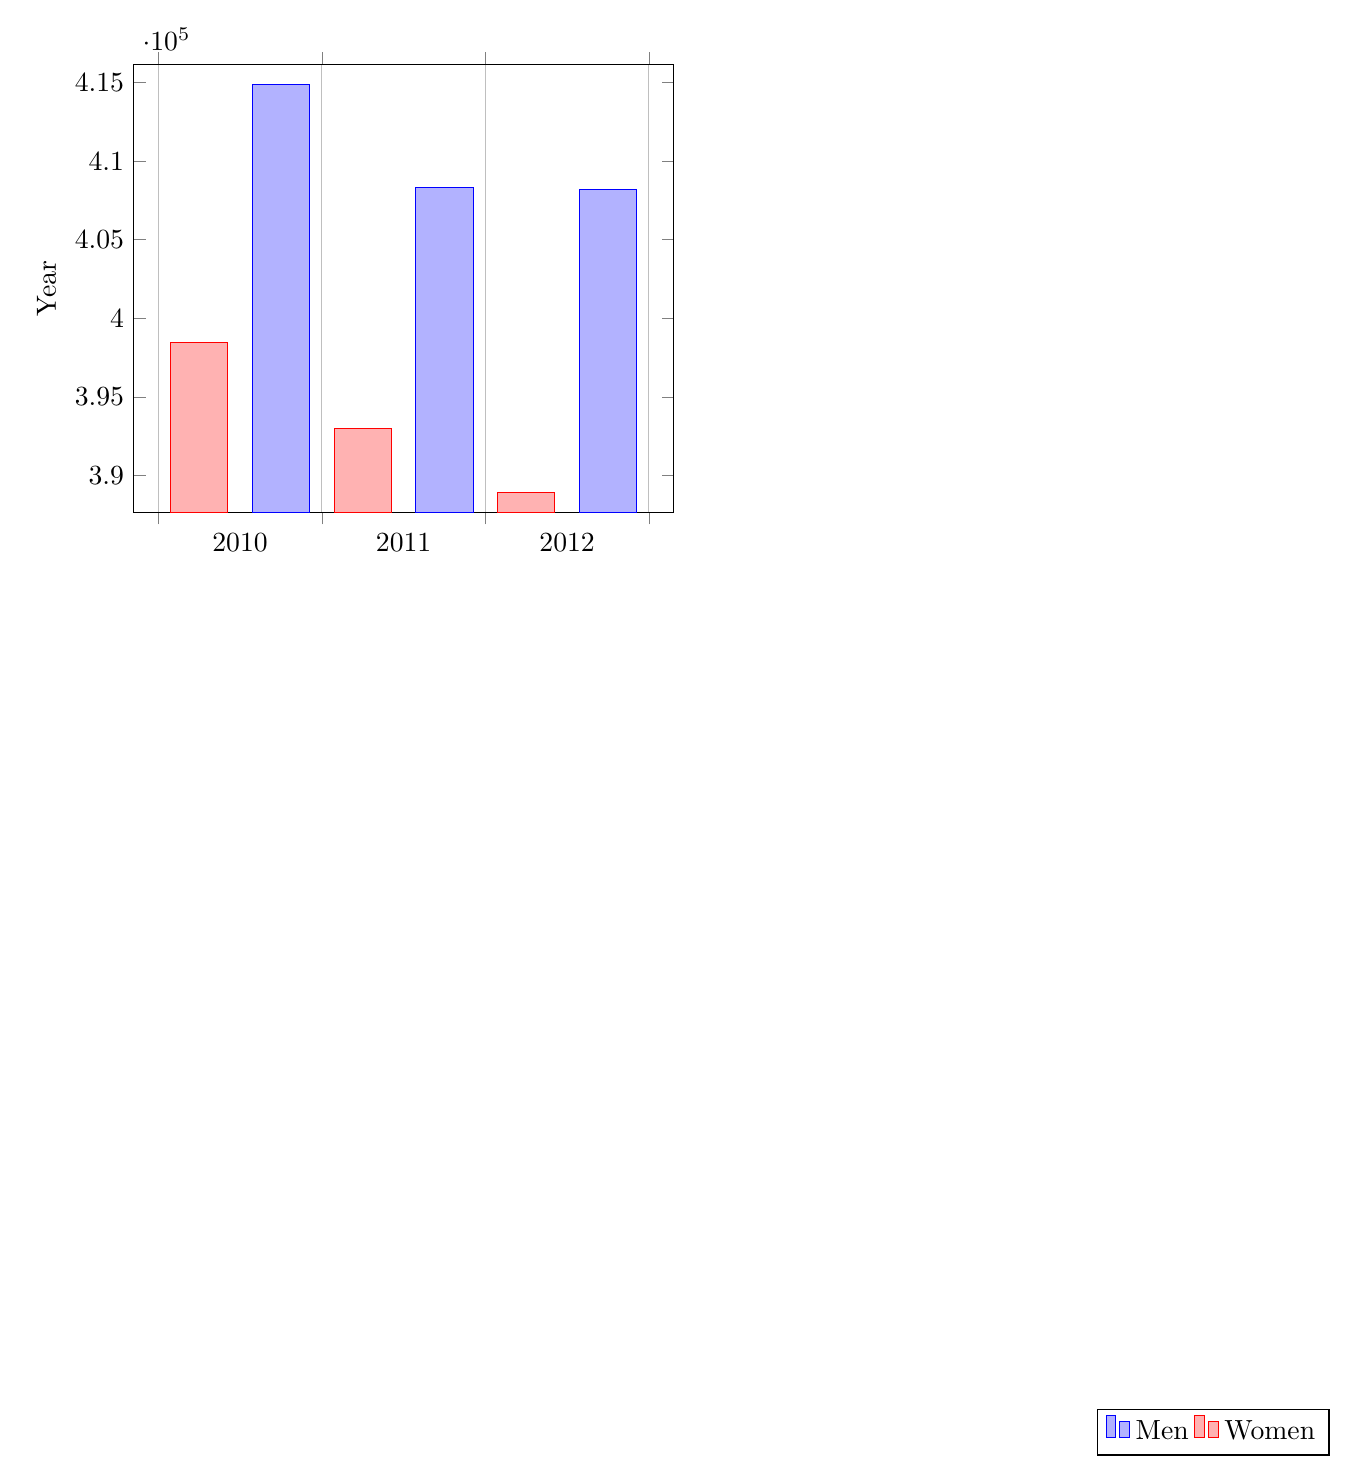
\begin{tikzpicture}
	\begin{axis}[
		x tick label style={
			/pgf/number format/1000 sep=},
		ylabel=Year,
		enlargelimits=0.05,
		legend style={at={(2,-2)},
			anchor=north,legend columns=-1},
		ybar interval=0.7,
		]
		\addplot 
		coordinates {(2012,408184) (2011,408348)
			(2010,414870) (2009,412156)};
		\addplot 
		coordinates {(2012,388950) (2011,393007) 
			(2010,398449) (2009,395972)};
		\legend{Men,Women}
	\end{axis}
\end{tikzpicture}

%----------------------------------------Solucion Desarrolladora----------------------------------------
\section{Soluci\'{o}n desarrolladora}
\begin{spacing}{1.5}
\end{spacing}
%----------------------------------------Objectivo general----------------------------------------------
\section{Objetivo general}
\begin{spacing}{1.5}
\end{spacing}
%----------------------------------------Objetivos especificos------------------------------------------
\section{Objetivos espec\'{i}ficos}
\begin{spacing}{1.5}
\end{spacing}


	
